\documentclass{beamer}
\usepackage{babel}
\usepackage[utf8]{inputenc}
\usepackage[T1]{fontenc}
\usepackage{graphicx}
\usepackage{stmaryrd}
\usepackage{xcolor}
\usepackage{tikz}
\usepackage{proof}
\usepackage{bussproofs}
\usepackage{listings}
\usepackage{amsmath}

\usetheme{Copenhagen}
\usefonttheme{professionalfonts}
\setbeamertemplate{navigation symbols}{}
\setbeamertemplate{headline}{}

\definecolor{delimiterColor}{HTML}{B65E47}
\definecolor{numberColor}{HTML}{FF0000}
\definecolor{commentColor}{HTML}{008000}
\definecolor{keyColor}{HTML}{002BFF}

\lstdefinelanguage{maude}
{
	breaklines=true,
	extendedchars=true,
	tabsize=2,
	frame=none,
	columns=fullflexible,
	showtabs=false,
	showstringspaces=false,
	showspaces=false,
	showstringspaces=false,
	identifierstyle={\ttfamily},
	keywordstyle={\color{keyColor}},
	ndkeywordstyle={\color{keyColor}},
	stringstyle={\color{delimiterColor}},
	commentstyle={\color{commentColor}},
	ndkeywords={Int, Bool, String},
	keywords={in, load, pr, protecting, sort, sorts, op, ops, var, vars,eq, cq, ceq,endfm, fmod, is, mod, endm, load, =, ==, =/=, euler, discreteswitch, nonaccurate, mp, rk4, accurate, init, exp, abs, true, false, nil, ctor, PhysicalEntityStar, PhysicalInteraction, PhysicalEntity, PhysicalEntityPC1, FlowSource, SysMan, effortDyn, flowDyn, Object, Oid, assoc, comm, id, DataCollector, Rat, NzNat, frac, trunc, if, else, class, load, homod, endhom, eof, var, vars, eq, op, ops, pr, inc, protecting, including, ceq, is, tomod, endtom, msg, rl, crl, trew, hfind, hsearch, tsearch, hmc, hrew, time, earliest, such, that, subclass, Prop, omod, sort, subsort, not, endom, fi, msgs, fmod, endfm, hfrew, then, mod, and, or, endm, endtm, in, out, set, trace, exclude, loop, show, using, stepsize, tick, Oid, Nat, Float, Configuration, String, NzNat},
	morecomment={[l]{***}},
	morecomment={[l]{---}},
}
\AtBeginSection[ ]
{
\begin{frame}{Outline}
    \tableofcontents[currentsection, hideallsubsections]
\end{frame}
}
\title{Conditional Rewriting Logic \& Maude}
\author{Niccolò Piazzesi}
\institute{
    Università degli studi di Pisa
}
\titlegraphic{
\includegraphics[width=2cm]{img/logo.png}}
\begin{document}

\frame{\titlepage}

\begin{frame}{Outline}
    \tableofcontents[hideallsubsections]
\end{frame}
\section{Introduction and main concepts}
\begin{frame}
    \frametitle{What is a concurrent system?}
    Modelling concurrent system is one of the most studied problems in Computer Science.

    \bigskip
    \pause
    Many proposed answers:\begin{itemize}
        \item Petri Nets 
        \item CCS
        \item CSP 
        \item Actors
        \item $\cdots$
    \end{itemize}
\end{frame}
\begin{frame}
    \frametitle{The need for unification}
    \pause
        \begin{block}{External fragmentation}
            Hard to relate different approaches, each with their own concepts, models and issues.
        \end{block}
    \pause 
    \begin{block}{Internal fragmentation}
        Sometimes, fragmentation appears also within a specific approach (e.g. how can we unify operational and denotational semantics of CCS?).
    \end{block}
    \pause
    \begin{block}{Concurrency in other areas}
        A related problem is the integration of concurrency with other paradigms ( OO, Functional, ...)
        without using complex \emph{ad hoc} solutions.
    \end{block}
\end{frame}

\begin{frame}
    
    Rewriting logic aim to resolve these issues with a two sides approach.
    \pause
    \begin{block}{Computational side}
        Computationally, rewriting logic is a \emph{semantic framework} where many different 
        models and languages can be represented and executed as \textbf{rewrite theories}. 
    \end{block}
    \pause
    \begin{block}{Logical side}
        Rewriting logic  is also a \emph{logical framework}, a model within which 
        many other logics and deduction procedures  can be modelled and reasoned about.        
    \end{block}
\end{frame}
\section{Foundations}
\begin{frame}
    \frametitle{A logic of action}
    The rules of rewriting logic resemble those of equational logic, but the meaning is very different.

    \begin{center}
        \textbf{Rewriting logic is a logic to reason about \emph{change} in a concurrent system, \emph{not about equality.}}
    \end{center}
\pause 

\bigskip 
Rewriting logic identifies \textbf{concurrent rewriting} with \textbf{deduction}.
\end{frame}

\begin{frame}
    \frametitle{Rewrite Theory}
    \begin{center}
        \resizebox{3cm}{!}{$(\Sigma, E, L, R)$}
    \end{center}
    
    \bigskip
    \begin{itemize}

        \item $\Sigma$: ranked alphabet of function symbols
        
        \item E: set  of $\Sigma$-equations 
       
        \item L: set of \emph{labels}
      
        \item R: set of pairs $R \subseteq L \times (T_{\Sigma, E}(\mathbf{X})^2)^+$
    \end{itemize}
    
    \pause
    \bigskip
    $T_{\Sigma,E}(\mathbf{X})$ denotes the $\Sigma-algebra$ of equivalence classes of $\Sigma-terms$ with variables in $\mathbf{X}$ modulo the equations E.
    
    \medskip
    Elements of R are called \emph{rewrite rules}.
\end{frame}

\begin{frame}

    An example: natural numbers with a nondeterministic choice operator 
    
    \pause
    \begin{itemize}
        \item $\Sigma = \{0,s\_,\_+\_,\_?\_\}$
        \pause
        \item $E = \{N + M = M + N\}$
        \pause
        \item R = 
            \vspace{-5mm}
            \begin{align*}
                &r1: N+0 \rightarrow N \\ 
                &r2: (s\ N) + (s\ M) \rightarrow s\ s\ (N + M) \\ 
                &r3: N ? M \rightarrow N \\ 
                &r4: N ? M \rightarrow M 
            \end{align*}
    \end{itemize}
\end{frame}
\begin{frame}
    \frametitle{Sequent entailment}
    \begin{center}
        \resizebox{3cm}{!}{$\mathcal{R} \vdash [t] \rightarrow [t']$}
    \end{center}

    \pause 
    \vspace{2cm}
    A rewrite theory $\mathcal{R}$ \emph{entails} a \emph{sequent}
    $ [t] \rightarrow [t']$ \emph{iff} $[t] \rightarrow [t']$ can be obtained 
    by finite application of \emph{rules of deduction}.
\end{frame}
\begin{frame}[allowframebreaks]
    \frametitle{Rules of deduction}
    \scriptsize
    \begin{enumerate}
        \item \emph{Reflexivity}. For each $[t] \in T_{\Sigma,E}(\mathbf{X})$, 
            $$
            \infer[]{[t] \rightarrow [t]}{}
            $$
        \item \emph{Congruence}. For each $f \in \Sigma_n, n \in \mathbb{N}$,
            $$
            \infer[]{[f(t_1,\cdots,t_n)] \rightarrow [f(t_1',\cdots,t_n')]}{[t_1] \rightarrow [t_1']\ \cdots\ [t_n] \rightarrow [t_n']}            $$ 
        \item \emph{Replacement}. For each rule  
        \begin{align*}
            r&:[t(\overline{x})] \rightarrow [t'(\overline{x})]\ if \\
            &[u_1(\overline{x})] \rightarrow [v_1(\overline{x})] \wedge \cdots \wedge [u_n(\overline{x})] \rightarrow [v_n(\overline{x})]
        \end{align*}
        in $R$,
        \begin{prooftree}
            \alwaysNoLine
            \AxiomC{$[w_1] \rightarrow [w_1']$}
            \UnaryInfC{$[u_1(\overline{w}/ \overline{x})] \rightarrow [v_1(\overline{w}/ \overline{x})]$}
                \AxiomC{$\cdots$}
                \UnaryInfC{$\cdots$}
                    \AxiomC{$[w_n] \rightarrow [w_n']$}
                    \UnaryInfC{$[u_k(\overline{w}/ \overline{x})] \rightarrow [v_k(\overline{w}/ \overline{x})]$}
                \alwaysSingleLine
                \TrinaryInfC{$[t(\overline{w}/ \overline{x})] \rightarrow [t'(\overline{w}'/ \overline{x})]$}
        \end{prooftree}

        \item \emph{Transitivity}
        $$
        \infer[]{[t_1] \rightarrow [t_3]}{[t_1] \rightarrow [t_2] \quad [t_2] \rightarrow [t_3]} 
        $$
        \item \emph{Unconditional replacement}. For each 
        $$ r: [t(x_1,\cdots,x_n)] \rightarrow [t'(x_1,\cdots,x_n)]$$
        in R, 
        $$
        \infer[]{[t(\overline{w} / \overline{x} )] \rightarrow [t'(\overline{w'} / \overline{x})]}{[w_1] \rightarrow [w_1'] \quad \cdots \quad [w_n] \rightarrow [w_n']}
        $$
    \end{enumerate}
\end{frame}
\begin{frame}
    \frametitle{Concurrent rewriting}
    $\mathcal{R} = (\Sigma, E, L, R)$
    \small
    
    \pause
    \medskip
    A $(\Sigma, E)$ sequent $[t] \rightarrow [t']$ is called:\begin{itemize}
        \item a \emph{0-step concurrent $\mathcal{R}$-rewrite} iff it can be derived from $\mathcal{R}$ by finite application 
        of rules (1) and (2).
        \pause
        \item a \emph{one-step concurrent $\mathcal{R}$-rewrite} iff it can be derived from $\mathcal{R}$
        by finite application of rules (1)-(3), with at least one application of (3).
        \pause
        \item a \emph{concurrent $\mathcal{R}$-rewrite} iff it can be derived from $\mathcal{R}$ by finite application   of rules (1)-(4).
    \end{itemize}
\end{frame}
\begin{frame}
    $\mathcal{R} = (\Sigma, E, L, R)$
    \small
   
    \medskip
    $\mathcal{R}$ is \emph{terminating} if there is no infinite chain of one step rewrites.

    \medskip
    $[t']$ is an $\mathcal{R}-normal\ form$ of $[t]$ if $[t] \rightarrow [t']$ is an 
    $\mathcal{R}$-rewrite and there is no $[t'] \rightarrow [t'']$ one-step  $\mathcal{R}$-rewrite.
    

    
    \medskip
    $\mathcal{R}$ is \emph{Church-Rosser} or \emph{confluent} if
    \begin{figure}
        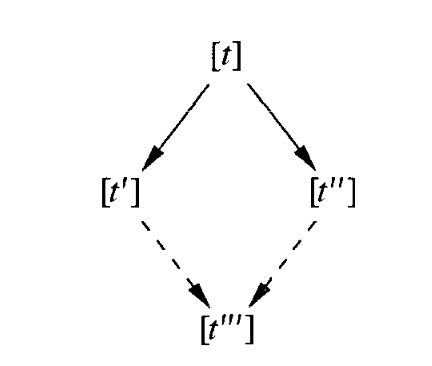
\includegraphics[scale=0.2]{img/churchrosser.png}
    \end{figure}
    
\end{frame}
\begin{frame}
    \frametitle{Reflection}

    Rewriting logic is \textbf{reflective}.

    
    \bigskip 
    There is a finitely presented rewrite theory $\mathbf{U}$ such that, for 
        any finitely presented rewrite theory $\mathbf{T}$ (including $\mathbf{U}$ itself) we have 
        the following equivalence:
       {\small $$
        T \vdash [t] \rightarrow [t'] \Longleftrightarrow \mathbf{U} \vdash  \langle \overline{T},\overline{[t]} \rangle  \rightarrow \langle \overline{T},\overline{[t']} \rangle
        $$ 
       }
        \bigskip
    Since $\mathbf{U}$ is representable in itself, we can create a "reflective tower" with any 
    number of levels of reflection:
    {\scriptsize
    $$T \vdash [t] \rightarrow [t'] \Leftrightarrow \mathbf{U} \vdash  \langle \overline{T},\overline{[t]} \rangle  \rightarrow \langle \overline{T},\overline{[t']} \rangle
    \Leftrightarrow\mathbf{U} \vdash  \langle \overline{\mathbf{U}},\overline{\langle \overline{T},\overline{[t]} \rangle} \rangle  \rightarrow  
    \langle \overline{\mathbf{U}},\overline{\langle \overline{T},\overline{[t']} \rangle} \rangle \cdots $$
    }
\end{frame}
\section{Semantic model}
\begin{frame}
    \begin{block}{What we have}
    $ R = (\Sigma, E, L, R)$

    \emph{Static description} of what a system can do.
        
    \end{block}
    
    \pause

    \begin{block}{What we want}
        \emph{Computational models} of the system behaviour (the \emph{meaning of the theory}).
    \end{block}

    \pause

    \begin{block}{Idea}
        Take advantage of the correspondence between  \emph{deductions} in rewriting logic 
        and \emph{concurrent computations}.
    \end{block}
\end{frame}
\begin{frame}
    \frametitle{The model }
    $
    R = (\Sigma, E, L, R)
    $

    \pause 
    \bigskip
    We seek a \textcolor{red}{category} $\mathcal{T_R(X)}$:\begin{itemize}
        \item Objects: \textcolor{blue}{$[t]_E$}
        \item Arrows: \textcolor{blue}{$[t_1]_E \xrightarrow{\pi} [t_2]_E$}
    \end{itemize}

    \pause 
    \bigskip
    \emph{Generator rules}: obtained from the rules of deduction (1)-(4) by decorating 
    the sequents with appropriate proof terms.
For simplicity we will consider the \emph{unconditional} case
\end{frame}
\begin{frame}
    \frametitle{Rules of generation}
    \scriptsize 
    \begin{enumerate}
        \item \emph{Identities.} For each $[t] \in T_{\Sigma, E}(\mathbb{X})$,
        $$
        \infer[]{[t]: [t] \rightarrow [t]}{}
        $$

        \item $\Sigma-structure$. For each $f \in \Sigma_n, n \in \mathbb{N}$,
        $$
        \infer[]
        {f(\alpha_1, \cdots, \alpha_n): [f(t_1, \cdots, t_n)] \rightarrow [f(t_1', \cdots, t_n')]}
        {\alpha_1: [t_1] \rightarrow [t_1'] \quad \cdots \quad \alpha_n:[t_n] \rightarrow [t_n']}
        $$

        \item \emph{Replacement.} For each rewrite rule 
        $r:[t(\overline{x})] \rightarrow [t'(\overline{x})]$
        in $\mathbb{R}$,
        \begin{prooftree}
            \AxiomC{$\alpha_1 : [w_1] \rightarrow [w_1']$}
                \AxiomC{$\cdots$}
                    \AxiomC{$\alpha_n : [w_n] \rightarrow [w_n']$}
                \TrinaryInfC{$r(\alpha_1,\cdots,\alpha_n) : [t(\overline{w}/ \overline{x})] \rightarrow [t'(\overline{w}'/ \overline{x})]$}
        \end{prooftree}

        \item \emph{Composition}
        $$
        \infer[]{\alpha;\beta : [t_1] \rightarrow [t_3]}{\alpha : [t_1] \rightarrow [t_2] \quad \beta : [t_2] \rightarrow [t_3]} 
        $$
    \end{enumerate}
\end{frame}
\begin{frame}

\large 
$\mathcal{P_R}(X)$ $\Rightarrow$ graph generated by rules (1)-(4)
\bigskip
\begin{itemize}
    \item Nodes: $T_{\Sigma,E}(X)$
    \item Arrows: $f \in \Sigma_n,n \in \mathbb{N}$,$\quad$ $r \in R$,$\quad$ $\_;\_$
\end{itemize}

\bigskip
\pause
$$Proof\ terms\ \Leftrightarrow\ Concurrent\ computations$$
\bigskip
\begin{center}
    \emph{When are two concurrent computations essentially the same?}
\end{center}
\end{frame}


\begin{frame}[allowframebreaks]
    \scriptsize
    \frametitle{$\mathcal{T_R}(X)$}
    Given a rewrite theory $\mathcal{R}$, the model $\mathcal{T_R}(X)$ is the quotient of 
    $\mathcal{P_R}(X)$ modulo the following equations:
    
    \begin{enumerate}
        \item \emph{Category}.
        \begin{enumerate}[a]
            \scriptsize
            \item Associativity. For all $\alpha,\beta,\gamma$,
            
            $(\alpha;\beta);\gamma = \alpha;(\beta;\gamma).$
            \item Identities. For each $\alpha: [t] \rightarrow [t']$,
            
            $\alpha;[t'] = \alpha,\quad [t];\alpha=\alpha.$
        \end{enumerate}
        \item \emph{Functoriality.}. For each $f \in \Sigma_n, n \in \mathbb{N}$,
        \begin{enumerate}[a]
            \scriptsize
            \item Preservation of composition. For all $\alpha_1,\cdots,\alpha_n,\beta_1,\cdots,\beta_n$,
            
            $f(\alpha_1;\beta_1,\cdots,\alpha_n;\beta_n) = f(\alpha_1,\cdots,\alpha_n);f(\beta_1,\cdots,\beta_n). $
            \item Preservation of identities.
            
            $ f([t_1],\cdots,[t_n])=[f(t_1,\cdots,t_n)].$
        \end{enumerate}
        \item \emph{Axioms} in $E$. For $t(x_1,\cdots,x_n)=t'(x_1,\cdots,x_n)$ an axiom in $E$, for all $\alpha_1,\cdots,\alpha_n$,
        $\quad t(\alpha_1,\cdots,\alpha_n)=t'(\alpha_1,\cdots,\alpha_n).$    
        \item \emph{Exchange}. For each rewrite rule $r:[t(\overline{x})] \rightarrow [t'(\overline{x})]$ 
    in $\mathbb{R}$,
        \begin{prooftree}
            \AxiomC{$\alpha_1 : [w_1] \rightarrow [w_1']$}
                \AxiomC{$\cdots$}
                    \AxiomC{$\alpha_n : [w_n] \rightarrow [w_n']$}
                \alwaysSingleLine
                \TrinaryInfC{$r(\overline{\alpha}) = r(\overline{[w]});t'(\alpha) = t(\overline{\alpha});r(\overline{[w']})$}
        \end{prooftree}
    \end{enumerate}
    
\end{frame}
\begin{frame}
    \textbf{Exchange law:} Rewriting at the top using $r$ and rewriting below using $\overline{\alpha}$
    are independent processes that can be done in any order or simultaneously.
    \pause
    \begin{figure}
        
        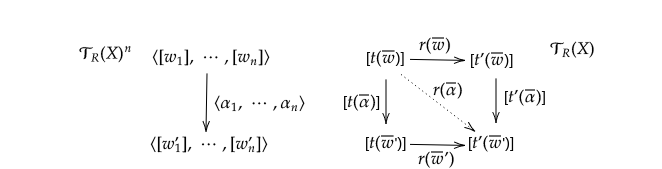
\includegraphics[width=\textwidth, height=\textheight,keepaspectratio]{img/nattr.png}
    \end{figure}
    \bigskip
   A rule $r$ is a natural transformation.



\end{frame}

\begin{frame}
    The construction $\mathcal{T_R}$ is very general, includes other constructions as particular cases.

    \pause
   
    $$\mathcal{R} : LTS \Rightarrow  \mathcal{T_R} : \underline{Path}$$

    \pause
    
    $$\mathcal{R} : \text{Petri nets} \Rightarrow  \mathcal{T_R} : \underline{Petri}$$

    \bigskip 
    \pause
$\mathcal{T_R}(X)$ is just one among many models for a rewrite theory $\mathcal{R}.$ Let's now see the general model.
\end{frame}
\begin{frame}
    \frametitle{$\mathcal{R}$-systems}
    \scriptsize
    Given a rewrite theory $\mathcal{R} = (\Sigma,E,L,R)$, an \emph{\textbf{$\mathcal{R}$-system $\mathcal{S}$}} is a 
    category $\mathcal{S}$ together with:
    \begin{enumerate}
        \item a family of functors $\{f_\mathcal{S}:\mathcal{S}^n \rightarrow \mathcal{S} | f \in \Sigma_n\}$
        satisfying the equations in $E$.
        \item for each rewrite rule $r:[t(\overline{x})] \rightarrow [t'(\overline{x})]$ in $R$, a natural transformation $r_\mathcal{S}$ from 
        $t_\mathcal{S}$ to $t'_\mathcal{S}$.
    \end{enumerate}

    An $\mathcal{R}-omomorphism\ F: \mathcal{S} \rightarrow \mathcal{S}'$ between two $\mathcal{R}$-systems is a 
    functor $F:\mathcal{S} \rightarrow S'$ such that:
    \begin{itemize}
        \item it is a $\Sigma$-algebra homomorphism,i.e, $f_\mathcal{S}*F = F^n*f_{\mathcal{S}'}$ for each $f \in \Sigma_n$
        \item for each rewrite rule $r:[t(\overline{x})] \rightarrow [t'(\overline{x})]\ if\ C$ in r we have: 
        $$ r_\mathcal{S} * F = F^n * r_{\mathcal{S}'} $$
    \end{itemize}

    \pause
    \bigskip
    $\underline{\mathcal{R}\text{-Sys}}$: category of models for the rewrite theory $\mathcal{R}$. 
    
    \medskip
    The homsets $\mathcal{R}\text{-Sys}(\mathcal{S},\mathcal{S'})$ are also categories.  
    The arrows are given by natural transformation $\delta:F \rightarrow G$ between $\mathcal{R}$-homomorphisms $F,G$ satisfying the identity 
    $\delta^n*f_{\mathcal{S}'}=f_\mathcal{S}*\delta$. 

    \medskip
    This makes $\underline{\mathcal{R}\text{-Sys}}$ a 2-category.
\end{frame}
\begin{frame}
    \frametitle{Computational view of $\mathcal{R}$-systems}
    \large
    \begin{align*}
        &System \quad &&\leftrightarrow  &&&\quad Category \\
        &State \quad &&\leftrightarrow &&&\quad  Object \\
        &Transition \quad &&\leftrightarrow &&&\quad Morphism \\ 
        &Procedure \quad &&\leftrightarrow &&&Natural \quad transformation \\ 
        &Distributed\ Structure\ &&\leftrightarrow &&& Algebraic\ Structure 
    \end{align*}
\end{frame}
\begin{frame}
    \large
    \frametitle{Initial and free $\mathcal{R}$-systems}
   
    $$\mathcal{T_R} =\ Initial\ Object\ in\ \underline{\mathcal{R}\text{-Sys}} $$ 


    \bigskip
    $$\mathcal{T_R}(X) =\ Free\ Object\ in\ \underline{\mathcal{R}\text{-Sys}} $$ 
    
\end{frame}
\begin{frame}
    \frametitle{Soundness and completeness}
    \scriptsize
    \begin{block}{Satisfaction}
        A sequent $[t(x_1,\cdots,x_n)] \rightarrow [t'(x_1,\cdots,x_n)]$ is \emph{satisfied} by 
        an $\mathcal{R}$-system $\mathcal{S}$ if there exists a natural transformation
        $$ \alpha: t_\mathcal{S} \Rightarrow t_\mathcal{S}'$$ 
        between the functors $t_\mathcal{S},t_\mathcal{S}':\mathcal{S}^n \rightarrow \mathcal{S}.$

        $$ S \models [t(x_1,\cdots,x_n)] \rightarrow [t'(x_1,\cdots,x_n)]$$
    \end{block}
\pause

For $\Theta \subseteq \underline{\mathcal{R}\text{-Sys}}$,
$$ \Theta \models [t(x_1,\cdots,x_n)] \rightarrow [t'(x_1,\cdots,x_n)]$$
if the sequent is satisfied by all $\mathcal{R}$-systems in $\Theta$.

\pause 
$$ \mathcal{R} \models [t(x_1,\cdots,x_n)] \rightarrow [t'(x_1,\cdots,x_n)]$$
if the sequent is satisfied by all $\mathcal{R}$-systems
\end{frame}
\begin{frame}
\begin{block}{Soundness}
    For $\mathcal{R}$ a rewrite theory,
    $$ \mathcal{R} \vdash [t(x_1,\cdots,x_n)] \rightarrow [t'(x_1,\cdots,x_n)]
    $$
    implies
    $$\mathcal{R} \models [t(x_1,\cdots,x_n)] \rightarrow [t'(x_1,\cdots,x_n)]
    $$ 
\end{block}
Proof is by induction on the depth of proof terms.
\end{frame}
\begin{frame}
    \scriptsize
    \begin{block}{Completeness}
        For $\mathcal{R}$ a rewrite theory,
        $$ \mathcal{R} \models [t(x_1,\cdots,x_n)] \rightarrow [t'(x_1,\cdots,x_n)]
        $$
        implies
        $$\mathcal{R} \vdash [t(x_1,\cdots,x_n)] \rightarrow [t'(x_1,\cdots,x_n)]
        $$ 

        \pause
        \bigskip
        \textbf{Proof}

        Since $\mathcal{R} \models [t(x_1,\cdots,x_n)] \rightarrow [t'(x_1,\cdots,x_n)]$, we have in particular that 
        $$ \mathcal{T_R}\{(x_1,\cdots,x_n)\} \models [t(x_1,\cdots,x_n)] \rightarrow [t'(x_1,\cdots,x_n)]$$
        which means that there is a natural transformation 
        \begin{align*}
         \alpha:& [t(x_1,\cdots,x_n)] \Rightarrow [t'(x_1,\cdots,x_n)] : \\
        &\mathcal{T_R}(\{x_1,\cdots,x_n\})^n \rightarrow \mathcal{T_R}(\{(x_1,\cdots,x_n)\}).
        \end{align*}
        When we instantiate $\alpha$ with objects $[x_1],\cdots,[x_n]$ we obtain the equivalence class  
        of proof terms 
        $$\alpha([x_1,\cdots, x_n]): [t(x_1,\cdots,x_n)] \rightarrow [t'(x_1,\cdots,x_n)].
        $$
        Therefore,the sequent is provable from $\mathcal{R}$, as desired.
    \end{block}
\end{frame}
\section{Maude}
\begin{frame}
    
\end{frame}
\begin{frame}
    \frametitle{What is Maude}
    \textbf{Maude}
    \begin{itemize}
        \pause
        \item Declarative programming language based on rewriting logic 
        \begin{itemize}
            \item Built by SRI international and University of Illinois
            \item Includes membership equational logic as a sublanguage based on OBJ3 
        \end{itemize}
        \pause
        \item Modelling of distributed systems 
        \pause 
        \item  Explicit state analysis 
        \begin{itemize}
            \item Simulation by rewriting 
            \item reachability analysis 
            \item LTL and LTLR model checking 
        \end{itemize}
        \pause 
        
        \item Unification 
        \item SMT solver
    \end{itemize}
\end{frame}
\begin{frame}{Outline}
    \tableofcontents[currentsection, currentsubsection,hideothersubsections]
\end{frame}
\begin{frame}[fragile]
    \frametitle{Functional Modules}
    \begin{lstlisting}[language=maude]
            fmod NAT-ADD is
                sort Nat .
             op 0 : -> Nat [ctor] .
             op s_ : Nat -> Nat  .
             op _+_ : Nat Nat -> Nat [assoc comm id: 0] .
             vars M N : Nat . --- This is a comment
             eq s N + s M = s s (N + M) .
            endfm

Maude> in nat-add.maude 

Maude> red s(s(0)) + s(0) .
result Nat: s s s 0

    \end{lstlisting}
\end{frame}
    \begin{frame}[fragile]
        \frametitle{Including modules}
        \begin{lstlisting}[language=maude]
            fmod NAT-LIST-CONSTR is
                protecting NAT-ADD .
                sort List .
             op nil : -> List [ctor] .
             op _ _ : List Nat -> List [ctor] .
             endfm
             *** "1 2 3" -> nil s(0) s(s(0)) s(s(s(0))) ***
        \end{lstlisting}
        
    \end{frame}


\begin{frame}[fragile]
    \frametitle{System modules}
    \scriptsize
    \begin{columns}
        \begin{column}{.5\textwidth}
            
            \begin{lstlisting}[language=maude]
 fmod VENDING-MACHINE-SIGNATURE is
    sorts Coin Item Marking .
    subsorts Coin Item < Marking .
 op __ : Marking Marking ->
    Marking [assoc comm id: null] .
 op null : -> Marking .
 op $ : -> Coin [format (r! o)] .
 op q : -> Coin [format (r! o)] .
 op a : -> Item [format (b! o)] .
 op c : -> Item [format (b! o)] .
endfm
            \end{lstlisting}
        \end{column}
        \begin{column}{.5\textwidth}
            \begin{lstlisting}[language=maude]
        load vending-machine-signature.maude
        mod VENDING-MACHINE is
            including VENDING-MACHINE-SIGNATURE .
            var M : Marking .
         rl [add-q] : M => M q .
         rl [add-$] : M => M $ .
         rl [buy-c] : $ => c .
         rl [buy-a] : $ => a q .
         rl [change] : q q q q => $ .
         endm
    \end{lstlisting}
        \end{column}
    \end{columns}
   \begin{lstlisting}[language=maude]
Maude>  rew [3] $ $ q q .        result Marking: $ $ $ q q q q
    
        frew[2] $ $ q q .  result (sort not calculated): ($ q) ($ $) q q                 
        
        search [4, 10] $ q q q =>+ a c c M:Marking 
            such that M:Marking =/= null .
        
        Solution 1 (state 108) M --> q q q q 
            ...
    \end{lstlisting} 
\end{frame}

\begin{frame}[fragile]
    \frametitle{Model checking}
    \scriptsize
    \begin{columns}
        \begin{column}{.6\textwidth}
            
            \begin{lstlisting}[language=maude]
mod MUTEX is
    sorts Name Mode Proc Token Conf .
    subsorts Token Proc < Conf .
 op __ : Conf Conf -> 
    Conf [ctor assoc comm id: none] .
 ops a b : -> Name [ctor] .
 op none : -> Conf [ctor] .
 op [_,_] : Name Mode -> Proc [ctor] .
 ops wait critical : -> Mode [ctor] .
 ops * $ : -> Token [ctor] .
 rl [a-enter] : $ [a, wait] => [a, critical] .
 rl [b-enter] : * [b, wait] => [b, critical] .
 rl [a-exit] : [a, critical] => [a, wait] * .
 rl [b-exit] : [b, critical] => [b, wait] $ .
endm
            \end{lstlisting}
        \end{column}
        \begin{column}{.4\textwidth}
            \begin{lstlisting}[language=maude]
    load mutex.maude
    load model-checker.maude
    
    mod MUTEX-PREDS is
        protecting MUTEX .
        including SATISFACTION .
        subsort Conf < State .
      op crit : Name -> Prop .
      op wait : Name -> Prop .
      var N : Name .
      var C : Conf .
      var P : Prop .
      eq [N, critical] C |= 
              crit(N) = true .
      eq [N, wait] C |=
              wait(N) = true .
      eq C |= P = false [owise] .
    endm
            \end{lstlisting}
        \end{column}
    \end{columns}
    
\end{frame}
\begin{frame}[fragile]
    \scriptsize
    \frametitle{Model checking}
    \begin{lstlisting}[language=maude]
         load mutex-preds.maude
        mod MUTEX-CHECK is
            protecting MUTEX-PREDS .
            including MODEL-CHECKER .
            including LTL-SIMPLIFIER .
         ops initial1 initial2 : -> Conf .
         eq initial1 = $ [a, wait] [b, wait] .
         eq initial2 = * [a, wait] [b, wait] .
        endm
***(
Maude> red modelCheck(initial1, [] ~(crit(a) /\ crit(b))) .
reduce in MUTEX-CHECK : modelCheck(initial1, []~ (crit(a) /\ crit(b))) .
rewrites: 22 in 10ms cpu (434ms real) (2200 rewrites/second)
result Bool: true

Maude> red modelCheck(initial2, [] ~(crit(a) /\ crit(b))) .
reduce in MUTEX-CHECK : modelCheck(initial2, []~ (crit(a) /\ crit(b))) .
rewrites: 22 in 0ms cpu (0ms real) (~ rewrites/second)
result Bool: true
)***
    \end{lstlisting}
\end{frame}
\begin{frame}[fragile]
    \scriptsize
    \frametitle{The meta level }
    Maude exploits the reflective nature of rewriting logic. 
    
    \bigskip
    Every Maude \emph{module} \textbf{$M$} can be represented  as 
    a \emph{term} \textbf{$\overline{M}$} of \emph{Sort} \textbf{Module}. 

    \begin{align*}
        t=f(a,g(b))& \quad  \text{module FOO}\\
            &\Downarrow \\ 
        \overline{t}='f[\{'a\}\text{Fo}&\text{o},'g[\{'b\}\text{Foo}]]
    \end{align*}

    \bigskip
    The META-LEVEL module efficienlty supports reflection, providing a number of functions to 
    perform metalevel computation in the universal theory 
    \begin{lstlisting}[language=maude]
op meta-apply : Module Term Qid Substitution MachineInt -> ResultPair .
op metaReduce : Module Term ~> ResultPair [special (...)] .
op metaRewrite : Module Term Bound ~> ResultPair [special (...)] .
op metaFrewrite : Module Term Bound Nat ~> ResultPair[special (...)] .    
\end{lstlisting}


\end{frame}
\begin{frame}[fragile]
    \scriptsize
    \frametitle{A meta example}
    \begin{figure}
        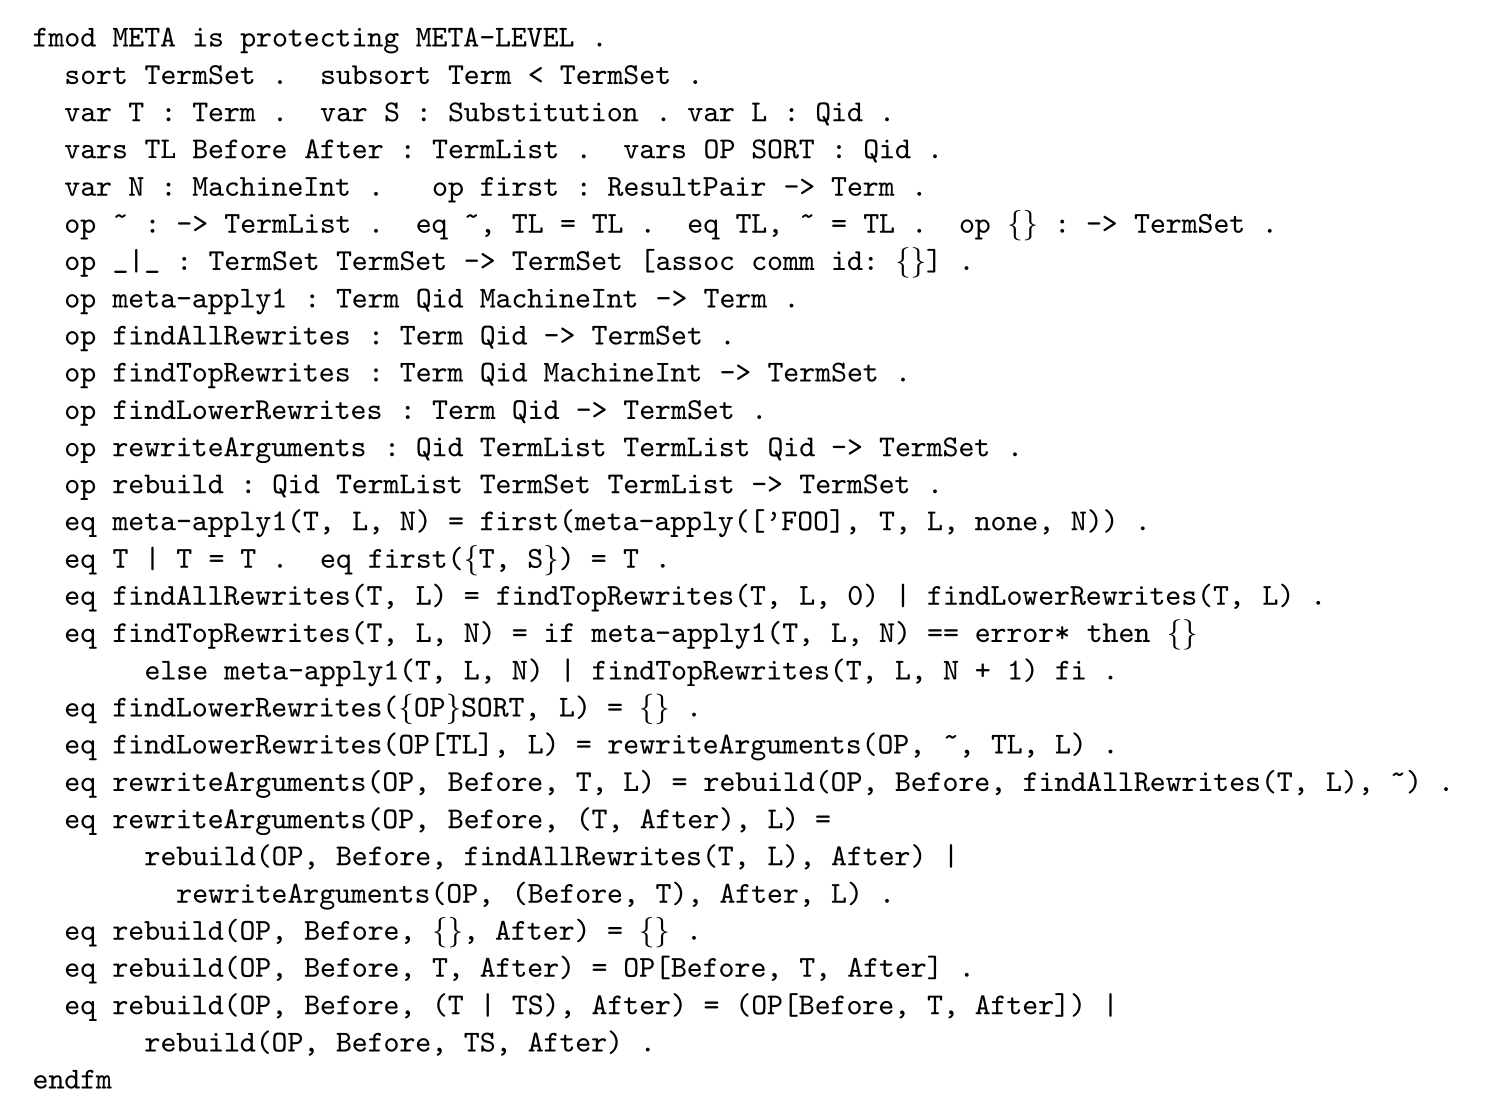
\includegraphics[width=\textwidth,height=.8\textheight, keepaspectratio]{img/meta.png}
    \end{figure}
\end{frame}
\begin{frame}[fragile]
    \scriptsize
    \frametitle{Objects in Full Maude}
    \begin{lstlisting}[language=maude]
    (omod ACCNT is 
        protecting QID .
        protecting MACHINE-INT .
        subsort Qid < Oid .
        class Accnt | bal : MachineInt .  
        
        msgs credit debit : Oid MachineInt -> Msg .  
        msg transfer_from_to_ : MachineInt Oid Oid -> Msg .  

        vars A B : Oid . 
        vars M N N' : MachineInt .  

     rl [credit] : credit(A, M) < A : Accnt | bal : N >
       => < A : Accnt | bal : (N + M) > .  
     crl [debit] : debit(A, M) < A : Accnt | bal : N >
       => < A : Accnt | bal : (N - M) >
          if N > M .  
     crl [transfer] : (transfer M from A to B)
       < A : Accnt | bal : N > < B : Accnt | bal : N' > 
       => < A : Accnt | bal : (N - M) > 
          < B : Accnt | bal : (N' + M) >
          if N > M . 
    endom)
    \end{lstlisting}
\end{frame}
\subsection{Maude by example}
\section{Applications}
\begin{frame}
    \frametitle{Applications}
    \begin{itemize}
        \item Formalization of programming languages 
        \begin{itemize}
            \item C
            \item Java, JVM
            \item Scheme
            \item K framework
            \item ...
        \end{itemize}
        \item Security: uncovering unknown attacks on web browsers 
        \item Logical framework 
        \begin{itemize}
            \item Barendregt's lambda cube 
            \item Linear logic 
            \item Modal logic
            \item ...
        \end{itemize}
        \item Biology : Pathway logic 
        \item Cloud transactions: \textcolor{red}{Google's Megastore}, Cassandra,...
    \end{itemize}

    For reference:

    http://maude.cs.illinois.edu/w/index.php/Applications
\end{frame}
\subsection{Megastore-CGC}
\begin{frame}{Outline}
    \tableofcontents[currentsection, currentsubsection,hideothersubsections]
\end{frame}
\begin{frame}
    \frametitle{Data in the cloud}
\begin{figure}
    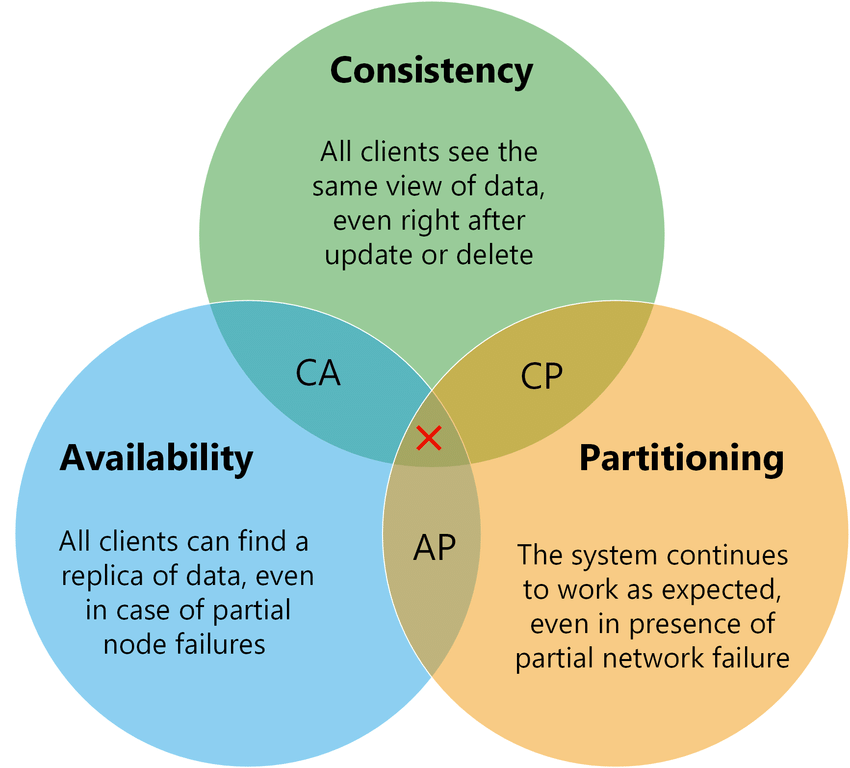
\includegraphics[width=.7\textwidth]{img/cap.png}
\end{figure}
\end{frame}
\begin{frame}
    \textbf{Availability AND Scalability} $\Rightarrow$ must replicate data

    How can i keep replicated data consistent?
    
    \bigskip
    Usual approach: \textcolor{red}{"Eventual consistency"}

    \bigskip
    Not ok for all applications (banking, commerce, medical systems,...)

    \bigskip
    Classical database transactions not well supported  in cloud computing, too expensive.
\end{frame}
\begin{frame}
    \frametitle{Google Megastore}
    \begin{itemize}
        \item Google's replicated data store.
        \item Billions  of read/write daily transactions.
        \item Adds (limited) support for transactions  in distributed data stores.   
    \end{itemize}
    \begin{figure}
        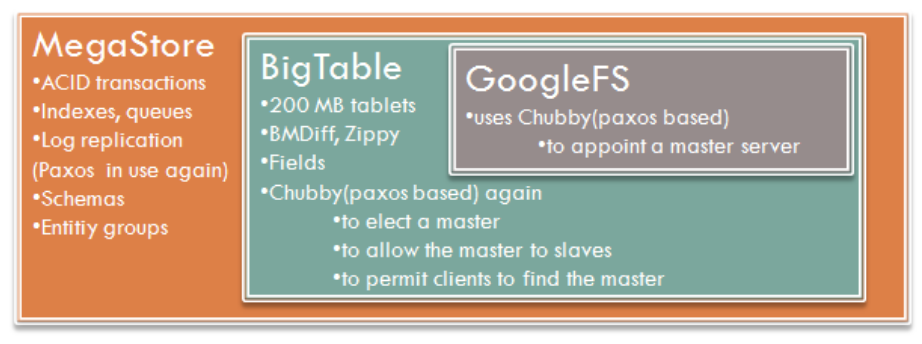
\includegraphics[width=\textwidth]{img/megastore.png}
    \end{figure}
\end{frame}
\begin{frame}
    \begin{itemize}
        \item Data divided into \textbf{entity groups.} 
        \item A single entity group is replicated across multiple \textbf{\emph{sites}}, managed by a \emph{\textbf{coordinator.}}
        \item \textbf{Replicated transaction log}  for each group.
        \item Two phase commits with a paxos-based protocol.
        \item Sites agree on next log entry if concurrent update.
    \end{itemize}
    \begin{figure}
        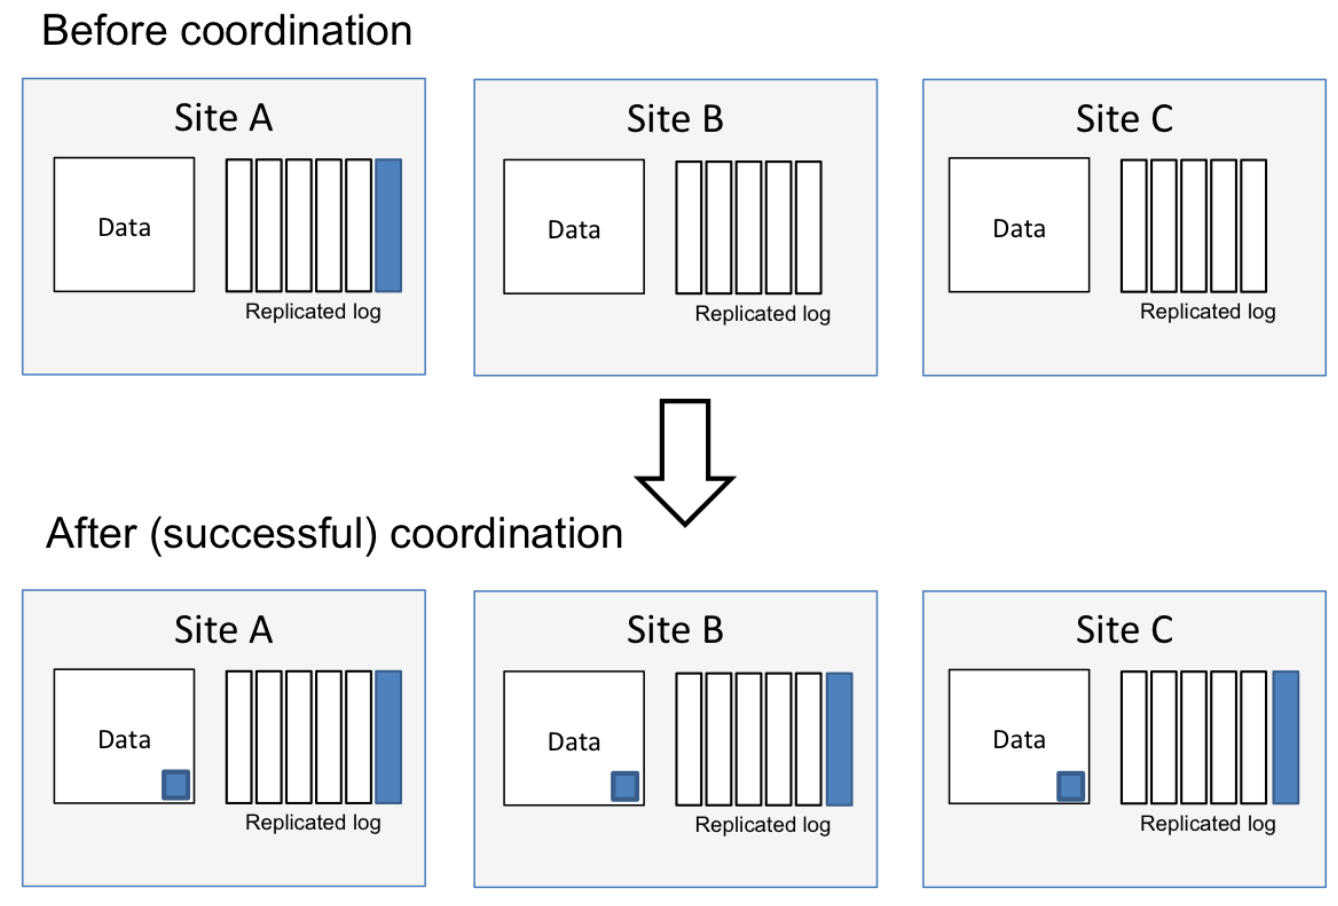
\includegraphics[width=\textwidth, height=.6\textheight,keepaspectratio]{img/paxos.png}
    \end{figure}
\end{frame}
\begin{frame}
    
    \large
    Megastore  guarantees consistency for transactions accessing a \textbf{single} entity group.

    \bigskip
    \textbf{Issues:}
    \begin{itemize}
        \item Original overview definition very informal, \textbf{really complex system}.
        \item No consistency guarantee if a transaction reads multiple entity groups.
        \begin{itemize}
            \item If you need consistency you could put all your data in a single entity group. 
            \item This could significantly worsen performance, concurrent updates works better 
            if the entity groups managed are smaller.
        \end{itemize}
    \end{itemize}
    
\end{frame}
\begin{frame}
    \frametitle{MegaStore CGC}
    \small
    Work by  Grov and $\ddot{\text{O}}$lveczky:
    \begin{itemize}
        \item Formalized Google MegaStore in Real-Time Maude.
        \begin{itemize}
            \item 56 rewrite rules (37 for fault tolerance).
            \item Use  of simulation and model checking to discover bugs during development.
        \end{itemize} 
        \item Introduced MegaStore CGC, an extension that provides consistency for transactions 
        accessing multiple entity groups. 
    \end{itemize} 
    
    \bigskip
    \begin{center}
    \textbf{Formal test driven development}
        \begin{enumerate}
            \item Express requirements as LTL formulas
            \item Develop Real Time Maude model 
            \item Test model through simulation and model checking 
            \item Analyse failures and modify the model
        \end{enumerate}
    \end{center}
\end{frame}
\begin{frame}[fragile]   

    \frametitle{Formalizing MegaStore} 
    \scriptsize   
    \begin{lstlisting}[language=maude]
class Site | entityGroups : Configuration, localTransactions : Configuration,
            coordinator : EntGroupLogPosPairSet, egOrderings : OrderClassUpdates,
            awaitingOrder : EntGroupUpdateList .

class EntityGroup | entitiesState : EntitySet, transactionLog : LogEntryList,
                    replicas : EntityGroupReplicaSet, proposals : PaxosProposalSet,
                    pendingWrites : PendingWriteList .

class Transaction | operations : OperationList, status : TransStatus,
                    reads : EntitySet, readState : ReadStateSet,
                    writes : OperationList, paxosState : PaxosStateSet .
    \end{lstlisting}
\end{frame}
\begin{frame}[fragile]
    \frametitle{A rewrite rule}
    \scriptsize
    \begin{lstlisting}[language=maude]
    crl [initiateCommit] :
        < SID' : Site |
            entityGroups EGROUPS,
            localTransactions : LOCALTRANS
                < TID : Transaction | operations : emptyOpList,
                                    writes : WRITEOPS, status : idle
                                    readState : RSTATE, paxosState : PSTATE > >
        =>
        < SID : Site |
            localTransactions : LOCALTRANS
                < TID : Transaction | paxosState : NEW-PAXOS-STATE,
                                    status : in-paxos > >
        ACC-LEADER-REQ-MSGS
    if EIDSET := getEntityGroupIds(WRITEOPS) /\
        NEW-PAXOS-STATE := initiatePaxosState(EIDSET, TID, WRITEOPS,
        SID, RSTATE, EGROUPS)
    /\ (createAcceptLeaderMessages(SID, NEW-PAXOS-STATE)) => ACC-LEADER-REQ-MSGS
        \end{lstlisting}
\end{frame}
\begin{frame}
    \scriptsize
    Performance was evalutated using Real Time Maude randomized simulations, which provides good performance estimates.

    
    \bigskip
    Simulation starts from realistic initial states and keep tracks of measures such as 
    average latency, number of commits, aborts, frequency of requests etc...
    \begin{figure}
        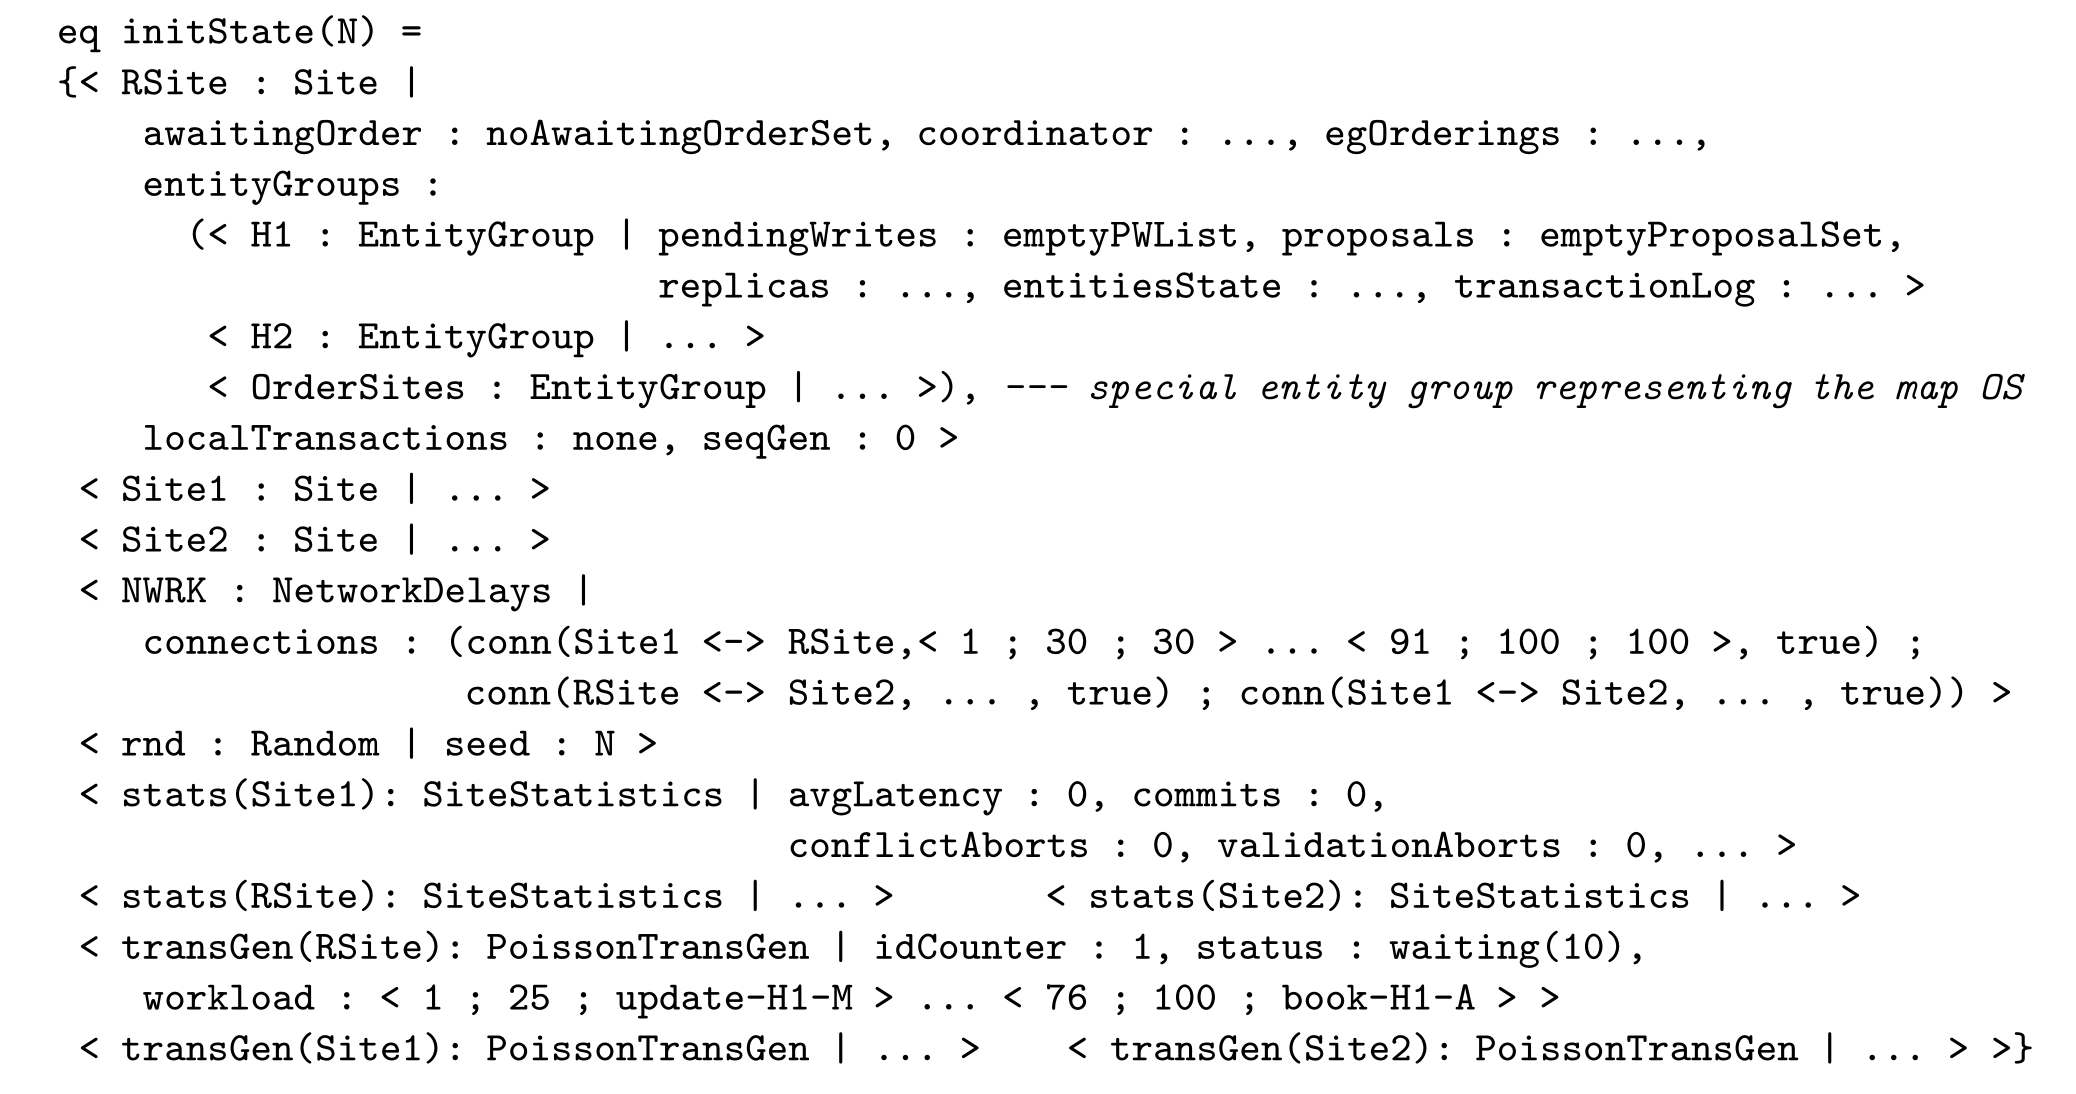
\includegraphics[width=\textwidth,height=\textheight,keepaspectratio]{img/init.png}
    \end{figure}
\end{frame}
\begin{frame}
\frametitle{Megastore-CGC}

    Observation:
    \begin{itemize}
        \item A site participates in all updates involving the entity groups it replicates 
        \item Implicit local ordering on these updates
    \end{itemize}  
            
    Idea:
    \begin{itemize}
        \item Select one site and make the ordering \textbf{explicit.}
        \item Site validates transactions on multiple entity groups before commit.
    \end{itemize}

    \emph{Ordering class} $\Rightarrow$ set of entity groups.

    \textbf{Ordering site} for each ordering class.
\end{frame}

\begin{frame}
    Megastore-CGC piggybacks its ordering and validation in the normal Megastore protocol.
    


    \bigskip
    Failure handling both for message loss AND ordering site failure.

    \bigskip
    No additional messages, mantains Megastore performance and fault tolerance. 

    \begin{figure}
        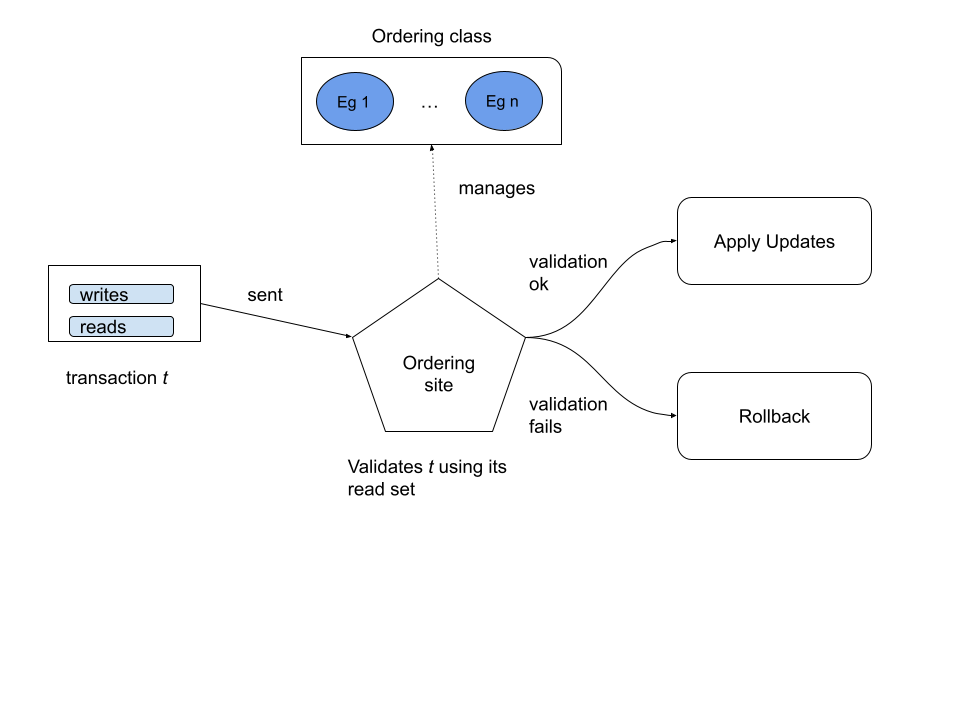
\includegraphics[width=\textwidth,height=\textheight,keepaspectratio]{img/validate.png}
    \end{figure}
\end{frame}

\begin{frame}[fragile]
    \frametitle{LTL requirements}
    System behaviour verification done via LTL model checking.
    
    \bigskip
    Desired Property: 
    \begin{lstlisting}[language=maude, basicstyle=\scriptsize]
    <> [] (allTransFinished /\ entityGroupsEqualOrInvalid
    /\ transLogsEqualOrInvalid /\ isSerializable)
    \end{lstlisting}

    All replicas are equal Property:
    \begin{lstlisting}[language=maude, basicstyle=\scriptsize]
    op entityGroupsEqualOrInvalid : -> Prop [ctor] .
    
    ceq {< S1 : Site | coordinator : eglp(EG1, LP) ; EGLP,
                    entityGroups :
                    < EG1 : EntityGroup | entitiesState : ES1 > EGS1 >
        < S2 : Site | coordinator : eglp(EG1, LP) ; EGLP,
                    entityGroups :
                    < EG1 : EntityGroup | entitiesState : ES2 > EGS2 >
    REST} |= entityGroupsEqual = false if ES1 =/= ES2 .
    
    eq {SYSTEM} |= entityGroupsEqualOrInvalid = true [owise] .
    \end{lstlisting}
\end{frame}
\begin{frame}
    \frametitle{Performance}
    Performance estimation done through Maude simulation, comparing MegaStore performance with Megastore-CGC.
    \begin{center}
        \textbf{(tfrew initState(10) in time <= 1000000 .)}
    \end{center}

    Result:
    \begin{center}
    \textbf{\{< stats(RSite): SiteStatistics | avgLatency : 94579/631, commitCount : 631,
conflictAborts : 171, validationAborts : 10, ... > ... \}}
    \end{center} 
\end{frame} 

\begin{frame}
    Analyzing results,  almost no difference in performance was found between Megastore and Megastore-CGC.
    \begin{figure}
        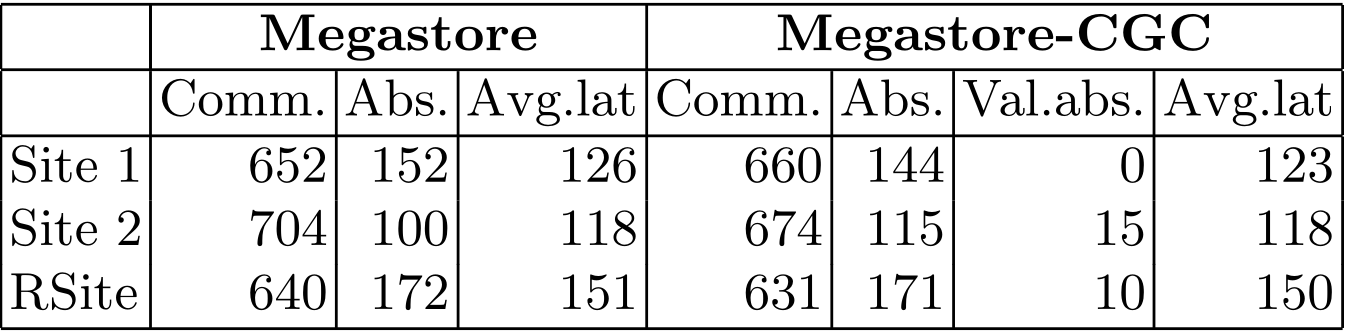
\includegraphics[width=\textwidth]{img/perf1.png}
        \end{figure}
    
    This is also true for "Megastore-friendly" transactions, those accessing 
    only one entity group.
    \begin{figure}
        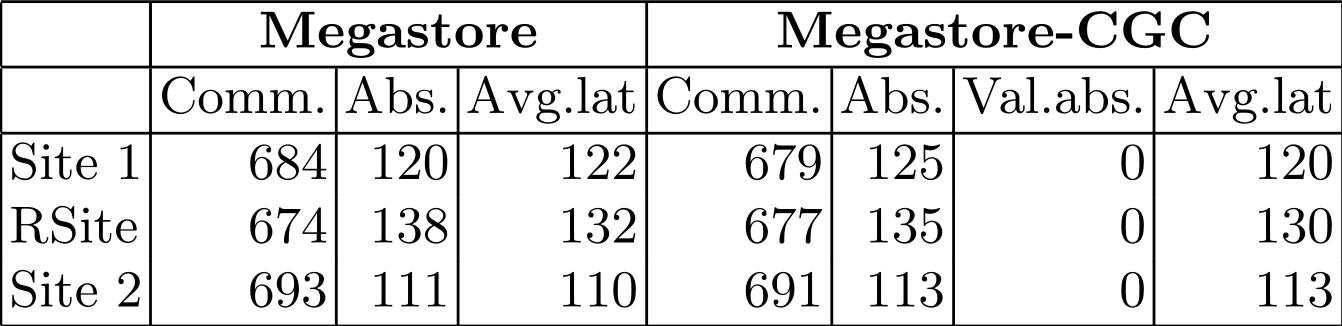
\includegraphics[width=\textwidth]{img/perf2.png}
    \end{figure}
\end{frame}

\begin{frame}
    \huge
    Thank you for your attention!
\end{frame}
\begin{frame}[allowframebreaks]
      \nocite{*}
        \frametitle{References}
        \bibliographystyle{unsrt}
        \bibliography{bib.bib}
\end{frame}

\end{document}